\chapter[SCP-078 罪恶感]{
    SCP-078 Guilt\\
    SCP-078 罪恶感
}

\label{chap:SCP-078}

\begin{figure}[H]
    \centering
    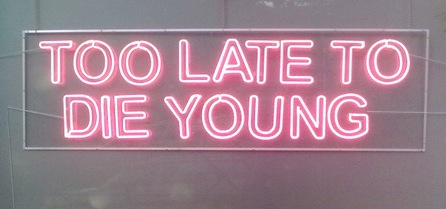
\includegraphics[width=0.5\linewidth]{images/SCP-078.jpg}
    \caption*{SCP-078,尚未进行收容前。}
\end{figure}

\bb{项目编号:}SCP- 078

\bb{项目等级:}Euclid

\bb{特殊收容措施:}SCP- 078挂在收容处墙上,并保持不通电的状态。收容处内唯一的插座应附有开关闸做为供给电力与否的控制,且除需进行相关实验,开关闸皆应设定在「关」。

进入SCP- 078收容处的人员,对于插座在处所内的安置位置及其控制开关闸位置皆应保持相当熟悉的状态,此条件为确保SCP- 078于意外开启的情形下,人员可以在闭眼状态将开关闸设定回「关」。

\bb{描述:}SCP- 078为一长约一米半的粉红色霓虹灯招牌,并展示字句“早死早超生(Too late to die young)”。这项SCP最早被发现在████████的████████镇区,经基金会的数据发掘协议程序纪录,发现该区在因饥饿及自我伤害而死亡的人数表现出不正常的高比例。

在未通电的状态下,SCP- 078没有任何变化,观察SCP- 078的人也不会有任何特殊反应。在开启后,观察SCP- 078时间在十秒以下及间接进行观察者也不会有特殊反应,此外,观察者若因不了解英文而无法理解SCP- 078展示的字句,该观察者也不会产生特殊反应。

然而,在开启状态下,能理解英文文句的观察者(下称受影响者)只要直接观察SCP-078十秒以上,他们在之后阅读任何手写文件时,会偶尔发现一些额外的字句,这些字句的书写风格皆与文件作者笔迹或文件格式完全相异(附录078 -01),并且字句内容会试图减轻受影响者因为某些事情或某些决定所产生的罪恶感。如一名D级人员就在他的手记中读到一句“她不听话,所以那是她应得的”,该员据信在一次激烈的争执中杀害了他的妻子。同时,██████博士在他写SCP-███的注记时,意外地发现一句“你的工作将会拯救人性”,该博士为了在基金会工作而离开了他的家人。

在观察SCP- 078十秒后,受影响者一开始会在心理上获得“极大地平静”,从而对受影响者产生助益。然而约于一星期内,观察者在手写文件上偶尔看见的额外字句,会从正向影响转变为负向影响。如██████博士即在观察两天后在个人手记上发现一句“他们从没用任何方式爱过你。”此外,字句内容也开始会为受影响者未感到罪恶感的其他行为编造正当理由,或是为受影响者已感知到具有罪恶感的行为辩护。不论是何者,受影响者都会重新思考该行为,并在之后自我合理化该行为及未来其他任何带有罪恶感的行为。随着时间过去, “行为正当化”的需求会不断增强,受影响者将会开始直接说出自己所做所为是合理的理由。

在一星期后,受影响者在执行任何基础生存必须(即呼吸睡眠等)之外的行为时,他们会变的异常计较细琐的部份,并且会为行为开始辩解“为何不做另一种行为”,从而导致受影响者产生神经病症症状。在两周后,受影响者将会无法正常进食,因为在咬下第一口食物后,受影响者会开始花几个小时来说明自己为什么第一口咬的是该食物的特定部份区域。除非进行营养剂注射,受影响者在这阶段之后通常会死于营养不良。目前已有█位D级人员及█位意外曝露在SCP- 078的研究人员已到此阶段,他们正接受营养剂注射维生,好进行寻找治疗此现像的方法,或其他更进一步的相关研究。

唯一会对受影响者产生更特殊影响的物件就是SCP- 078本身,当受影响者再次观察SCP- 078时,它展示的字句将会加深受影响者的罪恶感意识,且加深程度会依自初次观察后的相距时间提高。所有初次观察后,相隔一周再对SCP- 078进行观察的受影响者,皆试图自杀。

\bb{附录078-01:}D-19384,在曝露于SCP- 078后,于“最后”阶段时被处决。该名D级人员的书写文字为非常特别的图文混合风格。而在处决后,所有受影响者皆表示在看到额外字句时,曾看到相同于D-19384图文混合风格的书写文字。依此推测,死亡的受影响者,在非实体上可能会以某种方式被吸纳进SCP- 078。
